\chapter{Measurement of \texorpdfstring{$\thetaot$}{theta13}}
\label{ch:analysis}

The 3-flavor model of neutrino oscillation discussed in \cref{ch:intro}
was tested for goodness-of-fit against the Daya Bay observations,
and best-fit values for the oscillation parameters \thetaot{} and $\Delta m^2_{32}${}
were extracted.
For a \nuebar{} with energy $E_\nu$,
the probability that it will be detected as a \nuebar{}
after traveling a distance $L$ is predicted in the 3-flavor model as:

\begin{align}\label{eq:p_sur}
    \begin{split}
        P_\text{sur} = 1 &- \cos^4\thetaot\sin^22\theta_{12}\sin^2\Delta_{21} \\
                         &- \sin^22\thetaot(\cos^2\theta_{12}\sin^2\Delta_{31}
                     + \sin^2\theta_{12}\sin^2\Delta_{32}) \\
        \simeq 1 &- \cos^4\thetaot\sin^22\theta_{12}\sin^2\Delta_{21} \\
                 &- \sin^22\thetaot\sin^2\Delta_{ee},
\end{split}
\end{align}
where
$\Delta_{ji} \simeq 1.267 \Delta m^2_{ji} (\si{\eV}^2) L(\si{\m})/E_\nu (\si{\MeV})$,
and
$\Delta m^2_{ee} \simeq \cos^2\theta_{12}\left|\Delta m^2_{31}\right| +
\sin^2\theta_{12}\left|\Delta m^2_{32}\right|$.
As described in \cref{ch:intro},
the use of $\Delta m^2_{ee}$ to model the Daya Bay observations
is appropriate since the measurement is not sensitive
to the $O(\SI{1}{\percent})$ difference between $\Delta m^2_{31}$ and $\Delta m^2_{32}$.
Either form of \cref{eq:p_sur} can be used as a model
to compute the \nuebar{} survival probability
from the Daya Bay reactors to the near and far halls.
This analysis used the full 3-term model
assuming the normal mass ordering ($\Delta m^2_{32} > 0$)
when computing oscillation probabilities during the fit procedure.

To assess the validity of the 3-flavor model and extract the oscillation parameters'
best-fit values,
a comparison was made between the observed near-site and far-site \nuebar{} spectra.
The comparison relied on the number of observed events at the near halls (EH1 and EH2)
and $P_\text{sur}$ from the 3-flavor oscillation model
to predict the far-hall (EH3) observations
with minimal reliance on the intricacies of reactor operation modeling
and \nuebar{} production (\cref{sec:prediction}).
Reactor \nuebar{} models were used in the prediction
to determine the relative \nuebar{} flux
observed by each AD from each reactor core (\cref{sec:reactor}).
A \chisquare{} expression was created to quantify the agreement
between the prediction prediction and observations (\cref{sec:fitter}).

\section{Reactor \texorpdfstring{\nuebar{}}{antineutrino} model}
\label{sec:reactor}

The relative flux and spectrum of \nuebar{} from each reactor core was used
to adjust the predicted IBD spectrum at the far-hall ADs
based on how many \nuebar{}'s a particular near-hall AD was exposed to,
as described in detail in \cref{sec:prediction}.
The \nuebar{} production from each reactor was estimated from 3 fundamental contributions:
emission from fission products, corrections due to non-equilibrium effects,
and emission from spent nuclear fuel (SNF).
The resulting emission spectra specifying the spectrum per fission
were combined with knowledge of reactor power, fuel composition,
and energy released per fission
to estimate the total emitted \nuebar{} spectrum from each core.

The \nuebar{} spectrum was estimated for each of the four main fission isotopes
(\isotope[235]{U}, \isotope[238]{U}, \isotope[239]{Pu}, and \isotope[241]{Pu})
using the Huber \cite{reactor_huber} and Mueller \cite{reactor_mueller} models.
The Huber model was based on measurements of the total $\beta^{-}$ spectrum
for \isotope[235]{U}, \isotope[239]{Pu}, and \isotope[241]{Pu}
at the ILL reactor in the 1980s
\cite{ill_1,ill_2,ill_3}.
The Mueller model for \isotope[238]{U} used an \emph{ab initio} calculation
of the \nuebar{} spectrum
based on individual daughter isotope spectral measurements
accessible in the ENSDF nuclear database \cite{ensdf}.

Since the original ILL measurements relied on samples
which had been irradiated for at most 1.8~days,
they were not able to accurately measure
the effects of any daughter nuclides with decay times longer than a few hours.
Such isotopes would, however, reach equilibrium on the timescale
of a reactor fuel cycle of 12 to 18 months.
Corrections due to nonequilibrium effects, $c^{\text{ne}}_q(E)$
for each isotope $q$
were estimated using the ``450 day'' values from \cite{reactor_mueller},
shown in \cref{tab:noneq}.
For energy values between the reference energies,
a linear interpolation was used.
For energies below \SI{2}{\MeV}, a linear extrapolation was used
based on the \SIlist{2;2.5}{\MeV} corrections.
For energies above \SI{4}{\MeV}, a correction of 0 was used.

\begin{table}[ht]
    \centering
    \begin{tabular}[t]{lSSSSS}
        \toprule
        & \SI{2}{\MeV} & \SI{2.5}{\MeV} & \SI{3}{\MeV} & \SI{3.5}{\MeV}
                & \SI{4}{\MeV} \\
        \cmidrule(lr){2-6}
        Isotope $q$ & \multicolumn{5}{c}{Nonequilibrium correction $c^\text{ne}_q$ [\%]} \\
        \midrule
        \isotope[235]{U} & 5.7 & 4.4 & 1.5 & 0.7 & 0.1 \\
        \isotope[239]{Pu} & 2.1 & 1.7 & 0.5 & 0 & 0 \\
        \isotope[241]{Pu} & 1.9 & 1.5 & 0.5 & 0 & 0 \\
        \bottomrule
    \end{tabular}
    \caption[Nonequilibrium nuclide corrections]{
        Corrections to the predicted reactor \nuebar{} spectrum
        due to nonequilibrium nuclides
        for the three parent isotopes that required correction.
        The \isotope[238]{U} spectrum was computed differently
        from the others, as described in the text,
        and did not require a nonequilibrium correction.
    }
    \label{tab:noneq}
\end{table}

The \nuebar{} emission by spent nuclear fuel at the Daya Bay and Ling Ao reactor sites, $S^{\text{snf}}$,
was estimated using data from the power company \cite{snf}.
This additional flux was estimated to induce \SI{0.3\pm0.3}{\percent}
of the IBD interactions in each AD,
and contributed negligibly to the total uncertainty on \thetaot{}.
Given the negligible impact, a simplified model was used
where the spent nuclear fuel \nuebar{} flux was equally divided
among the six reactor cores and was constant over time.

Weekly average fission fractions $f_{q,w}$ and power levels $W_{\text{th},w}$ for each core
were obtained from the power company.
The energy emitted per fission for each isotope, $e_q$, was taken from
\cite{thermal_fission}.
Therefore, for each week, the total number of antineutrinos
of a given energy emitted from each core was computed,
given knowledge of a particular AD's livetime.
This analysis used data taken only when all EHs were operational;
thus within a given data-taking period (6-, 8-, or 7-AD period),
the reactor \nuebar{} average emission rate and spectrum was assumed to be identical
across all operational ADs.
The average rate of \nuebar{}'s produced by core $k$
during a particular data-taking period $d$ was
\begin{equation}\label{eq:reactor_spectrum_rate}
    \overline{\frac{d\phi_{k}^{d}}{dt}}(E) =
    \sum_{\substack{\text{weeks}\\w\in d}}\left\{
        \frac{T_{\text{DAQ},w} W_{\text{th},w}}{\sum_q f_{q,w} e_q}
        \sum_{\substack{\text{isotopes}\\q}}
    f_{q,w} S_q(E) \left[1+c_q^{\text{ne}}(E)\right]\right\} + S^{\text{snf}}(E).
\end{equation}
To obtain the total spectrum of \nuebar{}'s produced
during the livetime of a particular AD $i$,
the rates were converted to counts and summed over data periods:
\begin{equation}\label{eq:reactor_spectrum}
    \phi_{ik}(E) =
    T_{\text{DAQ},\,i}^{\text{6-AD}}
    \overline{\frac{d\phi_{k}^{\text{6-AD}}}{dt}}(E)
    + T_{\text{DAQ},\,i}^{\text{8-AD}}
    \overline{\frac{d\phi_{k}^{\text{8-AD}}}{dt}}(E)
    + T_{\text{DAQ},\,i}^{\text{7-AD}}
    \overline{\frac{d\phi_{k}^{\text{7-AD}}}{dt}}(E)
\end{equation}
The total numbers of \nuebar{}'s emitted between \SIlist{1.8;9.95}{\MeV}
from each core during the livetime of each AD are listed in \cref{tab:total_emitted}.
A typical \nuebar{} spectrum and the IBD cross section are shown
in \cref{fig:reactor_flux_xsec}.
The IBD cross section was computed \cite{ibd_xsec_note}
based on Eq.~(12) of \cite{ibd_xsec}
with constants from \cite{neutron_beta_theory,pdg2010}.

\begin{figure}
    \centering
    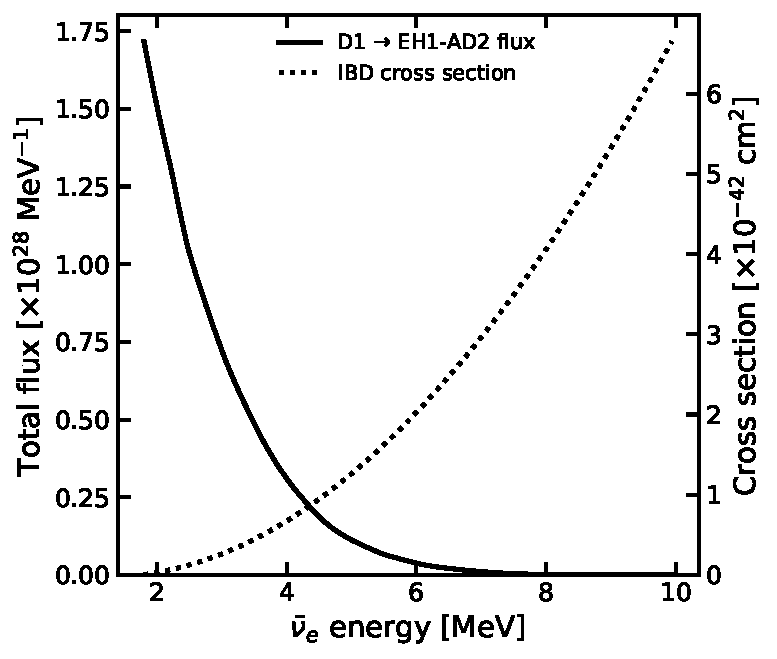
\includegraphics[width=0.7\textwidth]{ch_analysis/reactor_flux_xsec}
    \caption[Total reactor \nuebar{} flux and IBD cross section]{
        Total \nuebar{} flux produced by reactor core D1
        during the livetime of EH1-AD2,
        along with the IBD cross section.
    }
    \label{fig:reactor_flux_xsec}
\end{figure}

\begin{table}[ht]
    \centering
    \begin{tabular}[t]{lSSSSSS}
        \toprule
        & \multicolumn{6}{c}{Total predicted \nuebar{} flux [$\times10^{28}$]} \\
        \cmidrule(lr){2-7}
        & {D1} & {D2} & {L1} & {L2} & {L3} & {L4} \\
        \midrule
        EH1-AD1 & 1.93 & 1.99 & 1.99 & 1.98 & 2.01 & 1.91 \\
        EH1-AD2 & 2.23 & 2.28 & 2.24 & 2.27 & 2.24 & 1.18 \\
        \addlinespace
        EH2-AD1 & 2.23 & 2.29 & 2.25 & 2.27 & 2.24 & 1.19 \\
        EH2-AD2 & 2.03 & 2.01 & 2.01 & 2.03 & 1.98 & 2.00 \\
        \addlinespace
        EH3-AD1 & 2.23 & 2.28 & 2.24 & 2.27 & 2.24 & 1.18 \\
        EH3-AD2 & 2.23 & 2.28 & 2.24 & 2.27 & 2.24 & 1.18 \\
        EH3-AD3 & 2.23 & 2.28 & 2.24 & 2.27 & 2.24 & 1.18 \\
        EH3-AD4 & 2.03 & 2.01 & 2.00 & 2.03 & 1.97 & 2.00 \\
        \bottomrule
    \end{tabular}
    \caption[Total reactor \nuebar{} flux]{
        Total predicted \nuebar{} flux emitted from each core
        during the livetime of each AD.
    }
    \label{tab:total_emitted}
\end{table}

\section{Projection from near halls to far hall}
\label{sec:prediction}

The Daya Bay experiment was configured to use
identically-designed antineutrino detectors (ADs) at near and far sites
so that the measurements of the near and far ADs could be directly compared
with minimal systematic uncertainty due to detection efficiency
and reactor \nuebar{} modeling.
A predictive model was designed to implement the intuitive notion
that the observations at a near-hall AD can be used to predict
the observations at a far-hall AD \cite{p12e_fitter,p14a_fitter}.
This model of ``near-far projection'' estimates the contribution of each reactor core
to a given near AD's IBD sample,
then extrapolates each core's contribution to the far hall
based on oscillation effects, AD-reactor distance (baseline),
and differences in livetime, target mass and efficiency.
An alternative class of models,
where the observations at both near and far ADs
are predicted based on a model of reactor \nuebar{} emission
in addition to oscillation effects,
has been used for both nH and nGd analyses \cite{nh2016, ngd2016}.
In this thesis, the near-far projection model is used for the first time
to extract \thetaot{} from observations of neutron capture on hydrogen.


In the simplest configuration, with a single near observation,
a single far observation, and a single isotropic source of \nuebar,
the ratio of the number of observed far events $N_\text{f}$
to the number of observed near events $N_\text{n}$
depends on only a small set of quantities:
the detection efficiencies $\varepsilon_\text{n/f}$,
the number of target protons $N_\text{p,n/f}$,
the baselines $L_\text{n/f}$,
and the survival probability $P_\text{sur}(E_\nu, L_\text{n/f})$.
If the efficiencies, baselines, and number of target protons are well-determined,
then the near-far ratio becomes sensitive
to small changes in the survival probability via the formula \cite{ngd2016}

\begin{equation}\label{eq:near_far}
    \frac{N_\text{f}}{N_\text{n}} = \left(\frac{N_\text{p,f}}{N_\text{p,n}}\right)
    \left(\frac{L_\text{n}}{L_\text{f}}\right)^2
    \left(\frac{\varepsilon_\text{f}}{\varepsilon_\text{n}}\right)
    \left[\frac{P_\text{sur}(E_\nu, L_\text{f})}{P_\text{sur}(E_\nu, L_\text{n}}\right].
\end{equation}

In practice, the presence at Daya Bay of multiple \nuebar{} sources
located hundreds of meters apart
necessitated a more complex variant of \cref{eq:near_far}
that accounted for both the differences in reactor power and \nuebar{} spectrum over time,
and the two near halls, both of which observe \nuebar{}'s
in various stages of oscillation from all six reactor cores.
Given a set of observed IBD candidates at a near-hall AD,
the near-far projection model performs the following steps,
illustrated in \cref{fig:near_far_cartoon}:

\begin{figure}
    \centering
    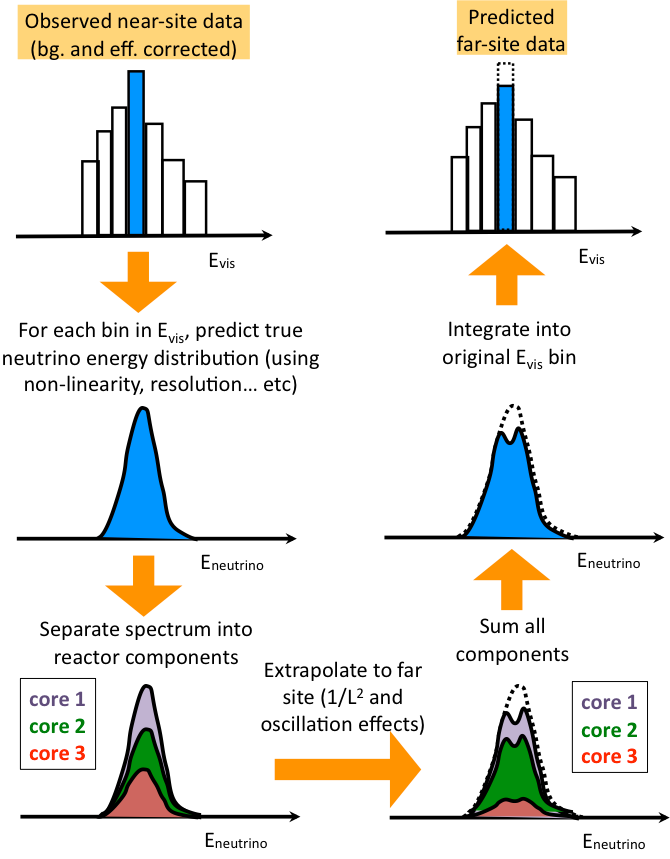
\includegraphics[height=0.5\textheight]{ch_analysis/near_far_cartoon}
    \caption[Diagram of near-to-far projection]{Illustration of the near-far projection procedure \cite{p12e_fitter}.}
    \label{fig:near_far_cartoon}
\end{figure}

\begin{enumerate}
    \item Subtract backgrounds from the near-hall measurement
        and adjust for detection efficiencies
    \item Convert the reconstructed prompt-energy spectrum
        into an estimated true \nuebar{} energy spectrum
    \item Predict the contribution of each reactor core
        to the observed \nuebar{} spectrum,
        including minor oscillation effects
    \item Extrapolate each core's contribution to the far hall ADs,
        accounting for oscillation effects and the AD-reactor baseline
    \item Convert the \nuebar{} energy back into a reconstructed energy
    \item Correct for the far AD's detection efficiency, backgrounds,
        target mass, and livetime
\end{enumerate}
The predicted spectrum at each far-hall AD can be compared
with the observed spectrum, as described in \cref{sec:fitter}.

In the following, the indices $i$ and $j$ refer to individual ADs,
$k$ and $l$ refer to reactor cores,
and $b$ refers to bins of reconstructed energy.

\subsection{Near-hall backgrounds and efficiencies}
\label{subsec:near_bg_eff}

The observed number of IBD candidates must be adjusted
to account for the backgrounds and efficiencies described in \cref{ch:event_selection}.
The backgrounds this analysis accounts for are
accidentals, \li{}/\he{}, fast neutrons, \amc{}, and radiogenic neutrons.
Efficiencies that can be measured precisely for each AD,
namely
the muon-veto livetime efficiency $\varepsilon_\mu$
multiplicity efficiency $\varepsilon_m$,
and target proton effective efficiency
$\varepsilon_{p,i}=N_{p,\text{AD }i}/N_{p,\text{EH1-AD1}}$,
are directly accounted for,
and are listed in \cref{tab:summary_event_selection}.
The remaining efficiencies, listed in \cref{tab:efficiency_summary},
are estimated for a generic or average AD and assigned a relative uncertainty.
Since the near-far projection is a relative measurement,
only deviations of individual ADs' efficiencies from the estimated mean value
impact the final prediction.
Therefore the remaining efficiencies are accounted for
by terms which quantify that potential difference.

Given a near-hall observation of $N_{\text{cand},i}^{(b)}$ IBD candidates
and $N_{\text{bg},i}^{(b)}$ estimated backgrounds in reconstructed energy bin $b$
of AD $i$,
the predicted number of IBDs is
\begin{equation}\label{eq:near_hall_bg_eff}
    N_{\text{IBD},i}^{(b)}(\thetaot, \Delta m^2_{32}) =
    \frac{N_{\text{cand},i}^{(b)}(1+\eta_{N,i}^{(b)})
        - \sum_u N_{\text{bg},i,u}^{(b)}(1+\eta_{B,i,u})}{
        \varepsilon_{\mu,i}\varepsilon_{m,i}\varepsilon_{p,i}(1+\epsilon_i)
        (1 + \eta_{\text{relE},i}\cdot a_{\text{relE},i}^{(b)}(\thetaot, \Delta m^2_{32}))
    },
\end{equation}
where $\eta_{N,i}^{(b)},\,\eta_{B,i,u},$ and $\epsilon_i$
represent fractional variations of
$N_{\text{cand},i}^{(b)},N_{\text{bg},i,u}^{(b)}$,
and the relative detection efficiency, respectively,
within their assigned uncertainties.
The relative energy scale (\cref{subsec:rel_energyscale})
is accounted for by a separate AD-dependent parameter $\eta_{\text{relE},i}$,
the fractional deviation of a given AD's energy scale
from the average for all ADs.
The parameter $a_{\text{relE},i}^{(b)}(\thetaot, \Delta m^2_{32})$
represents the fractional change to a given bin of reconstructed energy
due to the relative energy scale changing by $1\sigma \sim \SI{0.5}{\percent}$.
Its dependence on a given AD and the oscillation parameters is
due to the baseline-dependent distortion of the IBD spectrum
induced by neutrino oscillation.
The values for $a_{\text{relE},i}^{(b)}(\thetaot, \Delta m^2_{32})$ were determined using
the Individual Event Simulation dataset (\cref{sec:thu_toymc}).
The factor $(1 + \eta_{\text{relE},i}\cdot a_{\text{relE},i}^{(b)}(\thetaot,\Delta m^2_{32}))$
accounts for changes of
both shape and normalization (i.e.\ prompt-energy cut efficiency)
of the prompt spectrum
due to differences in the relative energy scale between ADs.
In practice $\eta_{N,i}^{(b)},\epsilon_i$ and $\eta_{\text{relE},i}$
were implemented as nuisance or pull parameters
so they could be adjusted during fitting.

The dependence of prompt-energy efficiency on oscillation parameters
discussed in \cref{subsec:prompt_energy}
should be applied at this stage for conceptual consistency.
However, the effect for a given AD, represented as $\delta_{p,ik}(\thetaot, \Delta m^2_{32})$,
depends on contributions from all 6 reactor cores,
so the inclusion of these factors is postponed
until they can be applied to each reactor core's contributions
individually in \cref{subsec:flux_fraction}.

The resulting $N_{\text{IBD},i}^{(b)}(\thetaot, \Delta m^2_{32})$ represents
the estimated number of IBD interactions in AD $i$,
reconstructed energy bin $b$,
including those which occurred during muon or multiplicity vetoes,
but not those which failed the prompt- and delayed-energy cuts
or the coincidence distance-time (DT) cut,
corrected for AD-to-AD differences in all cut efficiencies
number of target protons (target mass),
and energy scale.
Its dependence on the oscillation parameters
is very weak and is due to the relative energy scale uncertainty.


\subsection{Extracting the true \texorpdfstring{\nuebar{}}{antineutrino} spectrum}
\label{subsec:reco_to_true_energy}

The true \nuebar{} energy spectrum observed by the near halls
is required to compute oscillation probabilities.
The conversion from reconstructed to true energy
is impacted not only by the energy resolution and calibration
but also by the nonlinearities described in \cref{subsec:abs_energyscale}.
A detector response matrix was created
using the Individual Event Simulation (\cref{sec:thu_toymc})
by binning simulated events based on the true incoming \nuebar{} energy
and the reconstructed energy of the prompt event,
as shown in \cref{fig:drm}.
The simulation was configured so that the incident \nuebar{} energy
was drawn from the expected reactor \nuebar{} spectrum,
weighted by the IBD cross section \cite{ibd_xsec,ibd_xsec_note}.
For each bin of reconstructed energy,
a probability function was constructed
which described the spectrum of incident \nuebar{}'s
attributable to the IBDs in that reconstructed energy bin,
given the results of the simulation.
This probability was adjusted to account for
oscillation effects and so depended on \thetaot{} and $\Delta m^2_{32}${}
as well as the location of each AD relative to the reactor cores.
The normalized detector response matrix
showing probabilities for each bin of true and reconstructed energy for EH1-AD1
is shown in \cref{fig:drm_norm}.
A representative sample of probability functions
for individual bins of reconstructed energy
is shown in \cref{fig:drm_pdfs}.
The bins of true \nuebar{} energy had widths of \SI{0.05}{\MeV},
so for convenience, the true energy bins will be referred to
using function notation: $f(E_\text{true})$
refers to the value of $f$ in the bin containing true energy $E_\text{true}$.

\begin{figure}
    \centering
    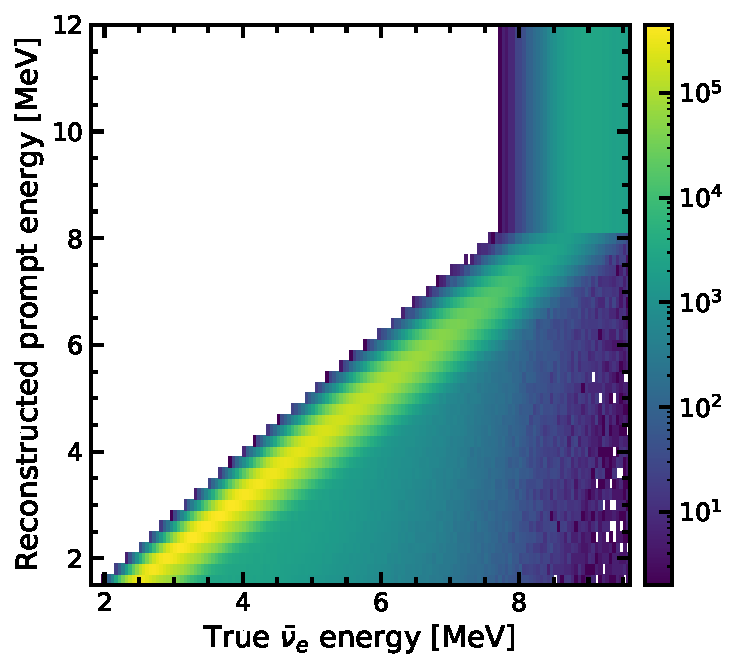
\includegraphics[width=0.5\textwidth]{ch_analysis/detector_response_raw}
    \caption[Detector response matrix]{
        Detector response matrix obtained from simulation.
        The color of each bin indicates the number of simulated IBD events
        with true \nuebar{} energy and reconstructed prompt energy
        corresponding to that bin.
    }
    \label{fig:drm}
\end{figure}

\begin{figure}
    \centering
    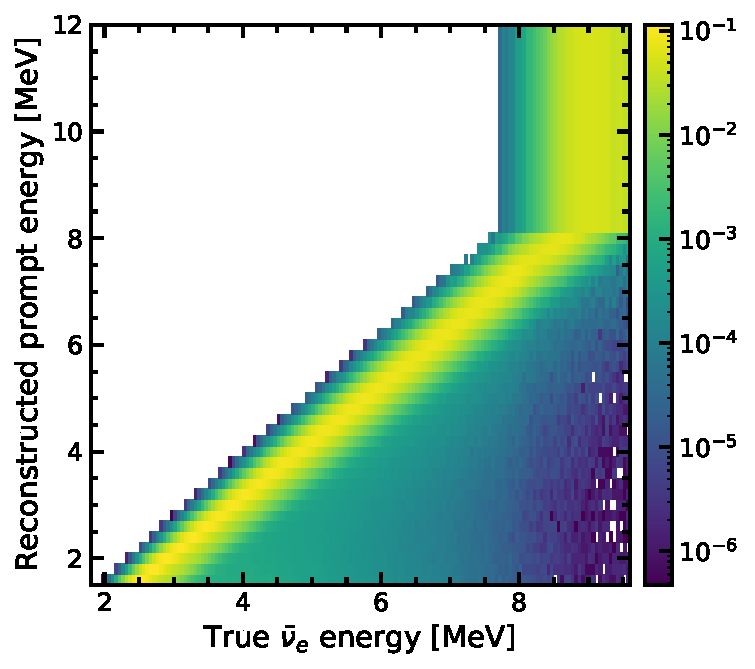
\includegraphics[width=0.5\textwidth]{ch_analysis/detector_response_norm}
    \caption[Detector response matrix, row-normalized]{
        Row-normalized detector response matrix
        showing $f^{(b)}_\text{DRM}(E_\text{true})$
        for EH1-AD1 using the best-fit \thetaot{}.
        The color of each bin indicates the probability
        of an IBD being caused by an \nuebar{} with the corresponding true energy,
        given that the event was observed with the corresponding prompt energy.
        Each row sums to unity by construction.
    }
    \label{fig:drm_norm}
\end{figure}

\begin{figure}
    \centering
    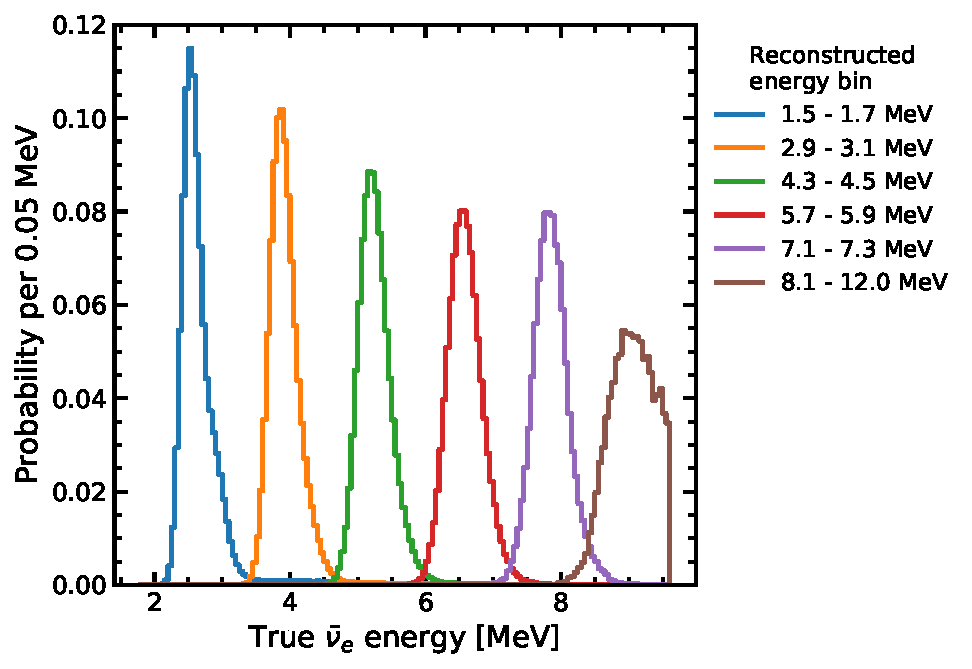
\includegraphics[width=0.7\textwidth]{ch_analysis/detector_response_pdfs}
    \caption[Individual rows of normalized detector response matrix]{
        Individual rows from the normalized detector response matrix
        showing the true \nuebar{} energy probabilities
        ($f^{(b)}_\text{DRM}(E_\text{true})$)
        for a representative sample of reconstructed prompt energy bins.
        The bin contents for each curve sum to unity by construction.
    }
    \label{fig:drm_pdfs}
\end{figure}

Given the near-hall AD observations,
a separate true \nuebar{} spectrum was computed
for each bin of reconstructed energy for each near-hall AD $i$ as
\begin{equation}\label{eq:drm}
    N_i^{(b)}(E_{\text{true}}) = N_{\text{IBD},i}^{(b)}
    \cdot f_{\text{DRM},i}^{(b)}(E_{\text{true}}; \thetaot, \Delta m^2_{32}),
\end{equation}
where $f_{\text{DRM},i}^{(b)}(E_{\text{true}}; \thetaot, \Delta m^2_{32})$ is the probability
that an event in reconstructed energy bin $b$
of AD $i$
was caused by a \nuebar{} with true energy in the same \SI{0.05}{\MeV}
energy bin as $E_{\text{true}}$.

The true-energy spectra derived from the various reconstructed energy bins
were never combined or mixed;
thus each reconstructed energy bin can be considered as an independent measurement
of the near-far ratio.
\Cref{subsec:true_to_reco_farhall} describes the procedure at the far hall
for converting from the true \nuebar{} energy back into reconstructed prompt positron energy.
For notational convenience, the subscript in $E_{\text{true}}$ will be omitted
in the subsequent sections,
and all energies should be assumed to be true \nuebar{} energies;
the prompt reconstructed energy is specified by the bin index $b$.

This methodology was used instead of the traditional method of
inverting the detector response matrix
because the process of inverting the matrix was numerically unstable.
Since variations in the detector response were highly constrained
to \SI{0.5}{\percent} in \cref{subsec:rel_energyscale},
the resulting true \nuebar{} spectra were meaningful when compared between ADs.
A thorough discussion of this procedure is given in \cref{ap:drm}.

\subsection{Separating near-hall observation into reactor components}
\label{subsec:flux_fraction}

Each AD observed \nuebar{}'s originating from all six reactor cores.
The near-far projection model decomposes each observation
of true \nuebar{} spectra $N_i^{(b)}(E)$
(from reconstructed energy bin $b$ of AD $i$)
into IBD contributions $N_{ik}^{(b)}(E)$ from each reactor core $k$,
where $\sum_k N_{ik}^{(b)}(E) = N_i^{(b)}(E)$.
The fraction of IBDs in near-hall AD $i$
(reconstructed energy bin $b$)
due to \nuebar{}'s from core $k$ is known as the flux fraction.

The flux fractions can be determined
by comparing each core's \nuebar{} flux $\phi_{ik}$ (\cref{eq:reactor_spectrum})
to the total from all reactors and
accounting for the $1/L^2$ dependence of isotropic \nuebar{} emission
and minor oscillation effects:
\begin{equation}\label{eq:flux_fraction}
    f_{ik}(E;\thetaot,\Delta m^2_{32}) = \frac{
        \phi_{ik}(E)(1+\alpha_k) P_\text{sur} (L_{ik}, E;\thetaot,\Delta m^2_{32})/L_{ik}^2
    }{
    \sum_l \phi_{il}(E)(1+\alpha_l)P_\text{sur}(L_{il}, E;\thetaot,\Delta m^2_{32})/L_{il}^2
    },
\end{equation}
where the sum in the denominator is over all cores.
The $\alpha_k$ and $\alpha_l$ parameters
encode the fractional uncertainty of the reactor flux normalization
(due to uncertainty in the reactor power)
and are implemented as nuisance parameters in the fitter in \cref{sec:fitter}.
The flux fractions depend only on true \nuebar{} energy
and are independent of reconstructed energy.
Note that in principle the IBD cross section $\sigma_{IBD}(E)$
should be included ($\phi \to \sigma_{IBD}\phi$),
but this factor is common to all cores (and all ADs)
and does not impact the ratio $f_{ik}$.
(\cref{sec:thu_toymc,subsec:reco_to_true_energy}).

The flux fraction is less sensitive to reactor \nuebar{} model uncertainties and biases
common to all cores.
Only uncertainties that are uncorrelated between cores
impact the prediction.

The number of IBDs observed at a given AD $i$ due to \nuebar{}'s from core $k$
can be computed from the flux fraction $f_{ik}$ as
\begin{equation}\label{eq:num_ibds_from_core_ij}
    N_{ik}^{(b)}(E) = \frac{
        f_{ik}(E) \times N_i^{(b)}(E).
    }{
        1 + \delta_{p,ik}(\thetaot, \Delta m^2_{32})
    },
\end{equation}
where the denominator is (belatedly) accounting for the dependence
of the prompt-energy efficiency on the \nuebar{} oscillations
between core $k$ and AD $i$,
as mentioned in \cref{subsec:near_bg_eff}
and described in detail in \cref{subsec:prompt_energy}.

\subsection{Extrapolating from near halls to far hall}
\label{subsec:extrapolation}

A prediction $F_{j,ik}^{(b)}(E)$ can be made of the number of expected IBDs
in reconstructed energy bin $b$
at far-hall AD $j$ due to reactor core $k$
given a particular event count at near-hall AD $i$ in reconstructed energy bin $b$.
The ratio of the far-hall prediction to the near-hall observation
is analogous to the ``near-far ratio''
that is the conceptual foundation
for the Daya Bay experimental design (\cref{eq:near_far}).
A distinct ratio exists for each combination of a near AD, a far AD and a reactor core,
for a total of $4 \times 4 \times 6 = 96$ ratios, also known as extrapolation factors
$e_{j,ik}$:
\begin{equation}\label{eq:extrapolation}
    e_{j,ik}(E;\thetaot,\Delta m^2_{32}) = \frac{
        \phi_{jk}(E)P_\text{sur}(L_{jk}, E;\thetaot,\Delta m^2_{32})/L_{jk}^2}{
        \phi_{ik}(E)P_\text{sur}(L_{ik}, E;\thetaot,\Delta m^2_{32})/L_{ik}^2
    }.
\end{equation}
Like the flux fractions, the extrapolation factors
do not depend on reconstructed energy.
Comparing \cref{eq:extrapolation} to the basic near-to-far ratio \cref{eq:near_far}, the extrapolation factors
do not account for differences in efficiency and number of target protons,
since those corrections are made in other steps of the near-far projection process
(\cref{subsec:near_bg_eff,subsec:far_bg_eff}).
On the other hand, the extrapolation factors do include a dependence on
differences in \nuebar{} exposure and detector livetime via the $\phi$ terms.
These differences arise due to slightly different DAQ livetimes
between the experimental halls
and a reactor flux which changes over time.
Note that the uncertainty in reactor flux normalization
($\alpha_k$ in \cref{eq:flux_fraction})
cancels in this ratio since the numerator and denominator represent the same reactor.

The predicted count of IBDs at far AD $j$ due to \nuebar{} from core $k$
based on the observation at near AD $i$ (all in reconstructed energy bin $b$) can be computed as
\begin{equation}\label{eq:far_true_core_pred}
    F_{j,ik}^{(b)}(E;\thetaot,\Delta m^2_{32}) = e_{j,ik}(E;\thetaot,\Delta m^2_{32}) \times
        N_{ik}^{(b)}(E;\thetaot,\Delta m^2_{32}) \times
        \left[1 + \delta_{p,jk}(\thetaot, \Delta m^2_{32})\right].
\end{equation}
The correction factor for the prompt-energy efficiency, $\delta_{p,jk}$, is included
to correct for oscillation effects between core $k$ and AD $j$,
and is described in detail in \cref{subsec:prompt_energy}.

The number of IBDs at a far AD including contributions from all cores,
but still based on a single near AD observation,
is simply the sum over all cores,
\begin{equation}
    F_{j,i}^{(b)}(E;\thetaot,\Delta m^2_{32}) = \sum_k F_{j,ik}^{(b)}(E;\thetaot,\Delta m^2_{32}).
\end{equation}

\subsection{Estimating the far-hall reconstructed spectrum}
\label{subsec:true_to_reco_farhall}

Independent predicted values $F_{j,i}^{(b)}(E)$ are obtained
for each bin of reconstructed prompt energy $b$.
This quantity, in full detail,
is the predicted number of IBDs at far-hall AD $j$
with true \nuebar{} energy $E$ in reconstructed energy bin $b$,
based on the observed number of IBDs at near-hall AD $i$
in reconstructed energy bin $b$.
Naively, the conversion from true to reconstructed energy
should be performed by applying the detector response matrix
from \cref{subsec:reco_to_true_energy}.
However, the \nuebar{} energy spectrum was not obtained
through inversion of the response matrix;
the alternate, PDF-based method was used.
With this method, the \nuebar{}'s do not model physical \nuebar{}'s with energy $E$.
Rather, they represent fictitious entities which always
lead to IBDs in the reconstructed energy bin $E_\text{rec}$,
and which are parametrized by a quantity $E$ that determines
the projection from a near AD to a far AD.
Thus the predicted ``events'' represented by a particular
$F_{j,i}^{(b)}(E)$ will all, by definition,
manifest as IBDs in reconstructed energy bin $b$,
and the total expected number of IBDs in bin $b$ becomes
\begin{equation}
    F_{j,i}^{(b)}(\thetaot,\Delta m^2_{32}) = \sum_E F_{j,i}^{(b)}(E;\thetaot,\Delta m^2_{32}),
\end{equation}
with the sum taken over the finely-binned true energy values
used in the detector response matrix and PDFs.

\subsection{Comparing with far-hall values}
\label{subsec:far_bg_eff}

To compare the predicted number of IBDs $F_{j,i}^{(b)}$
at far AD $j$ due to near AD $i$
to an actual observation at far AD $j$,
the prediction must account for far-hall backgrounds and efficiencies.
Additionally, there are multiple near-hall ADs
and hence multiple predictions for a single far-hall observed value,
but it is desirable to have a single prediction for each observation
to make use of the statistical methods in \cref{sec:fitter}.

To account for backgrounds and efficiencies at the far ADs,
the reverse of \cref{eq:near_hall_bg_eff} is applied:
\begin{align}\label{eq:far_hall_bg_eff}
    \begin{split}
        F_{\text{pred},j,i}^{(b)}(\thetaot,\Delta m^2_{32})
        = &F_{j,i}^{(b)}(\thetaot,\Delta m^2_{32})
            \varepsilon_{\mu,j}\varepsilon_{m,j}\varepsilon_{p,j}
            (1 + \epsilon_j)
            \left[1 + \eta_{\text{relE},j}\cdot
            a_{\text{relE},j}^{(b)}(\thetaot,\Delta m^2_{32})\right] \\
          &+ \sum_{\substack{u \in \text{bkg.}\\\text{sources}}}
        N_{\text{bg},j,u}^{(b)}(1 + \eta_{B,j,u}).
    \end{split}
\end{align}
The prompt-energy efficiency's dependence on oscillation parameters
was accounted for in \cref{eq:far_true_core_pred},
and the remainder of the prompt-energy efficiency difference between ADs
is due to relative energy scale differences,
represented by the $a_{\text{relE},j}^{(b)}$ parameters.
The resulting predicted numbers of IBD candidates
are directly comparable to each other (i.e. based on different near ADs)
and to the observed far-hall AD values.

\subsection{Summary of near-far projection}
\label{subsec:model_summary}

The steps of the near-far projection procedure can be combined into a single formula.
This formula gives the prediction for the number of observed events
in far-hall AD $j$ based on a given near-hall AD:
\begin{multline}\label{eq:full_prediction}
    F_{\text{pred},j,i}^{(b)}(\thetaot,\Delta m^2_{32}) =
    \Bigg\{
    \Big[N_{\text{cand},i}^{(b)}(1 + \eta_{N,i}^{(b)}) - N_{\text{bg},i}^{(b)}
          + \sum_{\substack{u \in \text{bkg.}\\\text{sources}}}
      N_{\text{bg},i,u}^{(b)}(1 + \eta_{B,i,u})\Big]\bigg. \\
    \times \frac{
        \varepsilon_{\mu,j}\varepsilon_{m,j}\varepsilon_{p,j}
        (1 + \epsilon_j)
        \left[1 + \eta_{\text{relE},j}\cdot a_{\text{relE},j}^{(b)}
            (\thetaot,\Delta m^2_{32})\right]
    }{
        \varepsilon_{\mu,i}\varepsilon_{m,i}\varepsilon_{p,i}
        (1+\epsilon_i)
        \left[1 + \eta_{\text{relE},i}\cdot a_{\text{relE},i}^{(b)}
        (\thetaot,\Delta m^2_{32})\right]
    } \\
    \bigg.
    \times \sum_{E,k} \left[
        %e_{j,ik}(E; \thetaot,\Delta m^2_{32}) f_{ik}(E; \thetaot,\Delta m^2_{32})
    \frac{
        \phi_{ik}(E)(1+\alpha_k) P_\text{sur} (L_{ik}, E;\thetaot,\Delta m^2_{32})/L_{ik}^2
    }{
    \sum_l \phi_{il}(E)(1+\alpha_l)P_\text{sur}(L_{il}, E;\thetaot,\Delta m^2_{32})/L_{il}^2
    } \right. \\
    \times \frac{
        \phi_{jk}(E)P_\text{sur}(L_{jk}, E;\thetaot,\Delta m^2_{32})/L_{jk}^2}{
        \phi_{ik}(E)P_\text{sur}(L_{ik}, E;\thetaot,\Delta m^2_{32})/L_{ik}^2
    } \\
        \left.\times f_{\text{DRM},i}^{(b)}(E)
    \times \frac{
        1 + \delta_{p,jk}(\thetaot, \Delta m^2_{32})
    }{
        1 + \delta_{p,ik}(\thetaot, \Delta m^2_{32})
    } \right] \Bigg\} \\
          + \sum_{\substack{u \in \text{bkg.}\\\text{sources}}}
        N_{\text{bg},j,u}^{(b)}(1 + \eta_{B,j,u}).
\end{multline}
The dependence on \thetaot{} and $\Delta m^2_{32}${}
is contained primarily in the flux fraction and extrapolation factors via $P_\text{sur}$.
Additional minor oscillation effects come from the relative energy scale uncertainty
$a_\text{relE}$ and prompt-energy efficiency corrections $\delta_p$.
As mentioned in previous sections and discussed in detail in \cref{sec:fitter},
the $\eta,\,\alpha$ and $\epsilon$ variables represent nuisance parameters
that quantify the uncertainties on various model inputs,
including efficiencies, background estimates,
and the statistical uncertainty of the near-hall AD observations.

Some quantities present in \cref{eq:full_prediction}
appear in both the numerator and denominator of the reactor flux terms,
and thus do not impact the final prediction value.
Specifically, the numerator of the flux fraction term
is nearly equal to the denominator of the extrapolation factor term;
only the reactor power uncertainty $(1 + \alpha_k)$ does not cancel.
This is another manifestation of the weak dependence of the
relative near-to-far prediction
on the intricacies of the reactor \nuebar{} model.

\section{Statistical methods}
\label{sec:fitter}

Standard frequentist techniques were used to determine the best-fit parameters
and goodness-of-fit between the 3-flavor neutrino oscillation model
and the data observed by Daya Bay.
A \chisquare{} expression with nuisance parameters
was the primary tool for this analysis.
Variants of this technique have been used both in previous Daya Bay nH analyses
and in other Daya Bay results including nGd \thetaot{} analyses
and absolute reactor \nuebar{} flux and spectral measurements
\cite{ngd2016,nh2016,reactorflux2017,extractionreactorflux2019}.

The fit procedure compared the observed number of \nuebar{} candidates
in the 4 ADs at the far site to the prediction
given the near sites' observations, a particular value of \thetaot{},
and values for all nuisance parameters.
Since the observed values represent event counts,
a \chisquare{} expression using the maximum likelihood expression
for Poisson-distributed data was used.
The generic structure of such \chisquare{} expressions
can be derived from Eqs.~(39.16) and (39.17) of \cite{pdg} as:

\begin{equation}
    \label{eq:chisquare_generic}
    \chisquare(\boldsymbol{\theta};\boldsymbol{\eta}) = 2\sum_{i=1}^{n} \left(
        F_{\text{pred},i}(\boldsymbol{\theta};\boldsymbol{\eta}) - F_{\text{obs},i}
        + F_{\text{obs},i}\ln
        \frac{F_{\text{obs},i}}{F_{\text{pred},i}(\boldsymbol{\theta};\boldsymbol{\eta})}
        \right)
        +
        \sum_j \frac{\eta_j^2}{\tilde{\sigma}_{\eta,j}^2},
\end{equation}
where $F_{\text{obs},i}$ is the observed value for data point $i$;
$F_{\text{pred},i}$
is the model prediction for data point $i$
which depends on $\boldsymbol{\theta}$ (the model parameters of interest)
and $\boldsymbol{\eta}$
(the nuisance parameters);
and there are $n$ data points.

In this formulation, the nuisance parameters are dimensionless,
and in the model they each multiply a paired quantity $A_j$,
which intuitively represents the physically-relevant quantity
(such as a detection efficiency or background rate)
that the nuisance parameter introduces uncertainty for:
\begin{equation}
    A_j \to (1+\eta_j)A_j.
\end{equation}
Thus the $\eta_j$ can be interpreted as the relative deviation of $A_j$
from an expected or constrained value,
and the $\tilde{\sigma}_{\eta,j}$ are the (independently-determined)
\emph{relative} uncertainties of $A_j$
that set the scale for allowable values of $\eta_j$.
The values of $A_j$ remain fixed during the minimization procedure;
only the values of $\eta_j$ are tunable parameters in the fit.

The values of $\boldsymbol{\theta}$ and $\boldsymbol{\eta}$
that minimize \cref{eq:chisquare_generic}
provide the best-fit parameters of interest $\theta_i$,
while ensuring that the nuisance parameters $\eta_j$
remain small compared to their uncertainties.
Intuitively, when the best-fit value of $\eta_j$ is nonzero,
the model has preferred a deviation of the physical parameter $A_j$ from its estimated value;
large deviations penalize the \chisquare{} and so are discouraged.
If the model is a good description of the data,
then the distribution of the best-fit (minimum) $\chi^2$
over repeated hypothetical experiments
follows a $\chi^2$ distribution with
\begin{equation}\label{eq:ndf_def}
    \text{NDF} = n - \text{len}(\boldsymbol{\theta})
\end{equation}
degrees of freedom,
where $\text{len}(\boldsymbol{\theta})$ is the number of components of $\boldsymbol{\theta}$,
that is, the number of free parameters in the fit.
Note that introducing additional nuisance parameters
paired with penalty terms (i.e.\ the second summation in \cref{eq:chisquare_generic})
does not in general change the number of degrees of freedom.

\subsection{Fitter specification}
\label{subsec:fitter_specification}

For this analysis, each data point $F_{\text{obs},j}$
was the number of observed events passing all event selection criteria
(\cref{ch:event_selection})
in a particular far-hall AD $j$.
There are thus 4 observed data points:
\begin{equation}
    \mathbf{F}_{\text{obs}} =
    (F^{\text{obs}}_{\text{EH3-AD1}},
    F^{\text{obs}}_{\text{EH3-AD2}},
    F^{\text{obs}}_{\text{EH3-AD3}},
    F^{\text{obs}}_{\text{EH3-AD4}}).
\end{equation}
The use of the total number of events as the observation data points
is known as a rate-only analysis,
in contrast to the rate-plus-shape analysis, which would use
the count of events in each bin of reconstructed energy
as its observation data points.
The model prediction
$\mathbf{F}_{\text{pred}}(\boldsymbol{\theta};\boldsymbol{\eta})$
of the event counts for the far-hall ADs
is described in \cref{sec:prediction}.
Reconstructed prompt energy bins of size \SI{0.2}{\MeV} were used from \SIrange{1.5}{8.1}{\MeV},
and a single bin of size \SI{3.9}{\MeV} was used from \SIrange{8.1}{12}{\MeV}.
To obtain the total number of predicted events at a given far AD $j$
based on measurements at a given near AD $i$,
the individual bin predictions from \cref{eq:full_prediction} were summed:
\begin{equation}\label{eq:hybrid_rate_shape}
    F_{\text{pred},j,i}(\boldsymbol{\theta};\boldsymbol{\eta}) =
    \sum_b F_{\text{pred},j,i}^{(b)}(\boldsymbol{\theta};\boldsymbol{\eta})
\end{equation}
To obtain a single value for the prediction at a given far AD $j$
based on all of the near AD measurements,
the individual predictions were combined in an unweighted average:
\begin{equation}\label{eq:average_near}
    F_{\text{pred},j}(\boldsymbol{\theta};\boldsymbol{\eta}) =
    \frac{1}{4} \sum_i
    F_{\text{pred},j,i}(\boldsymbol{\theta};\boldsymbol{\eta}).
\end{equation}
A livetime-weighted average was considered,
but since the 4 near-AD predictions were highly consistent,
weighting the contributions had no substantial impact
on the extracted value of \thetaot{}.
The vector of predictions contains one component for each far-site AD:
\begin{equation}\label{eq:f_pred_vector}
    \mathbf{F}_\text{pred}(\boldsymbol{\theta};\boldsymbol{\eta}) =
    (
    F^{\text{pred}}_{\text{EH3-AD1}}(\boldsymbol{\theta};\boldsymbol{\eta}),
    F^{\text{pred}}_{\text{EH3-AD2}}(\boldsymbol{\theta};\boldsymbol{\eta}),
    F^{\text{pred}}_{\text{EH3-AD3}}(\boldsymbol{\theta};\boldsymbol{\eta}),
    F^{\text{pred}}_{\text{EH3-AD4}}(\boldsymbol{\theta};\boldsymbol{\eta})
    )
\end{equation}
This prediction vector depends on the observed event rates at the near halls (EH1 and EH2),
reactor power and fission fractions,
differing background rates for each AD,
conversion between reconstructed prompt energy and true \nuebar{} energy,
detection efficiencies,
and, of course, neutrino oscillation parameters.
The parameters of interest and nuisance parameters were defined as follows:
\begin{align}
    \begin{split}
        \boldsymbol{\theta} &= (\thetaot) \\
        \boldsymbol{\eta} &= (
            \boldsymbol{\alpha},
            \boldsymbol{\epsilon},
            \boldsymbol{\eta_{\text{relE}}},
            \boldsymbol{\eta}_B,
            \boldsymbol{\eta}_N,
            \boldsymbol{\eta_{\text{osc}}}),
    \end{split}
\end{align}
where the nuisance parameters are collected into smaller vectors.
The vector $\boldsymbol{\alpha}$ represents reactor \nuebar{} flux uncertainties,
$\boldsymbol{\epsilon}$ represents detection efficiency uncertainties
(except for those induced by the relative energy scale uncertainty),
$\boldsymbol{\eta_{\text{relE}}}$ represents the relative energy scale uncertainty
and associated efficiency uncertainty,
$\boldsymbol{\eta_B}$ represents background rate uncertainties for each background source,
$\boldsymbol{\eta_N}$ represents the statistical uncertainty
of the observed event rates at the near hall ADs,
and $\boldsymbol{\eta_{\text{osc}}}$ represents the uncertainty
of the externally-imposed oscillation parameters, $\theta_{12},\,\Delta m^2_{21},$
and $\Delta m^2_{32}${}.
The observations were not binned by energy,
thus this analysis could not extract
a precise measurement of $\Delta m^2_{32}$.
An input value of $\Delta m^2_{32} = \SI{2.471(70)e-3}{\eV\squared}$
was supplied from \cite{ngd2018}, and
the uncertainty in $\Delta m^2_{32}${} was implemented as a nuisance parameter.
The input values and uncertainties for $\theta_{12}$ and $\Delta m^2_{21}$
were taken from \cref{eq:current_values} \cite{pdg}.

The full listing of nuisance parameters
can be found in \cref{tab:systs}.
During the fitter validation study (\cref{subsec:fitter_validation}),
a negligible effect on the extracted value of $\sin^22\thetaot$
($\lesssim\SI{0.1}{\percent}$)
was found as a result of the systematic uncertainty
of the absolute energy scale, energy resolution,
and reactor \nuebar{} spectral shape.
Thus these quantities were not modeled using pull parameters,
and instead were assumed to be known to infinite precision.
These values all contributed to the detector response functions
(\cref{eq:drm});
correlated variations of the detector response
canceled to first order, as discussed in \cref{ap:drm}.

\begin{table}[ht]
    \centering
    \footnotesize
    \begin{tabular}[t]{lp{3.1cm}p{2.5cm}p{3.8cm}}
        \toprule
        Systematics source & Relative uncertainty
                          & Pull parameters
                          & Notes\\
        \midrule
        Reactor power & \SI{0.8}{\percent}
                      & 6 (1 per core) & \\
        Reactor spectrum & negligible
                         & 0
                         & see \cref{sec:lbnl_toymc} \\
        Detection efficiency & \SI{0.66}{\percent}
                             & 8 (1 per AD)
                             & Includes $\Delta N_p$, excludes prompt-energy efficiency \\
        Relative energy scale & \SI{0.5}{\percent}
                              & 8 (1 per AD) & Includes prompt-energy efficiency \\
        All other detector response & negligible
                                    & 0
                                    & see \cref{sec:lbnl_toymc} \\
        Accidental background rate & \SI{0.08}{\percent} to \SI{0.1}{\percent}
                                   & 8 (1 per AD)
                                   & \\
        \li{}/\he{} background rate &
        \SI{48}{\percent}, \SI{45}{\percent}, \SI{38}{\percent} for EH1, EH2, EH3
                                    & 3 (1 per EH) & \\
        Fast neutron background rate &
        \SI{8}{\percent}, \SI{13}{\percent}, \SI{19}{\percent} for EH1, EH2, EH3
                                     & 3 (1 per EH) & \\
        \amc{} background rate & \SI{50}{\percent}
                             & 1 & \\
        Radiogenic neutron bkg. rate & \SI{50}{\percent}
                                           & 8 (1 per AD) & \\
        Input mixing parameters &
        \SI{2.4}{\percent}, \SI{2.6}{\percent}, \SI{2.8}{\percent} for
        $\Delta m^2_{21},\theta_{12}, \Delta m^2_{32}$
                                & 3
                                & \\
        Near AD statistical uncertainty & $1/\sqrt{N_{\text{cand},i}^{(b)}}$
                                        & 136 (1 per bin per near AD)&\\
        \bottomrule
    \end{tabular}
    \caption[Systematics summary]{Systematic uncertainties and associated nuisance parameters.}
    \label{tab:systs}
\end{table}

The full \chisquare{} expression used in this analysis is:

\begin{align}\label{eq:chisquare_full}
    \begin{split}
        \chisquare(\thetaot;\boldsymbol{\eta}) &=
            2\sum_{\substack{j \in \\\text{far ADs}}}
        \left(
            F_{\text{pred},j}(\thetaot;\boldsymbol{\eta}) - F_{\text{obs},j}
            + F_{\text{obs},j}\ln
            \frac{F_{\text{obs},j}}{F_{\text{pred},j}(\thetaot;\boldsymbol{\eta})}
        \right) \\
            &+ \sum_{\substack{r \in \\\text{reactors}}}
                \frac{\alpha_r^2}{\tilde{\sigma}_R^2}
            + \sum_{\substack{d \in \\\text{all ADs}}}
            \left(
                \frac{\epsilon_d^2}{\tilde{\sigma}_D^2}
                + \frac{\nu_{\text{relE},d}^2}{\tilde{\sigma}_{\text{relE}}^2}
                + \sum_{\substack{u \in \text{bkg.}\\\text{sources}}}
                \frac{\eta_{B,d,u}^2}{\tilde{\sigma}_{B,d,u}^2}
            \right) \\
            &+ \sum_{\substack{d \in \\\text{near ADs}}}
            \sum_{b \in \text{bins}}
            \left(\frac{\eta_{N,d}^{(b)}}{\tilde{\sigma}_{\text{obs},d}^{(b)}}
            \right)^2
            + \frac{\nu_{\theta_{12}}^2}{\tilde{\sigma}_{12}^2}
            + \frac{\nu_{\Delta m^2_{21}}^2}{\tilde{\sigma}_{21}^2}
            + \frac{\nu_{\Delta m^2_{ee}}^2}{\tilde{\sigma}_{ee}^2}
    \end{split}
\end{align}

The fitter was implemented in software using the
\texttt{optimize.least\_squares} function from the SciPy Python package,
which relies on the Trust Region Reflective algorithm
to perform the \chisquare{} minimization \cite{scipy,trf_minimizer}.
This minimizer relies on the cost function (\chisquare{})
being a sum of squared terms,
and expects the results of each trial
to be an array of terms to be squared and summed.
The Poisson maximum-likelihood \chisquare{} expression
is not naturally represented as a sum of squares,
but it can be trivially rewritten to comply with this requirement
since each summand in the \chisquare{} expression of the form
$F_\text{pred}-F_\text{obs}+F_\text{obs}\ln\frac{F_\text{obs}}{F_\text{pred}}$
is always greater than or equal to 0.
On occasion, this expression evaluated to a slightly-negative value
due to the finite precision of floating-point arithmetic.
These cases were handled by assigning the expression the value 0,
an approximation that was accurate to better than one part in $10^{10}$.

The implementations of the model described in \cref{sec:prediction}
and the $\chi^2$ expression described in \cref{sec:fitter}
(collectively, the ``fitter'')
were validated against the Fake Experiment Simulation
designed for the nGd analysis \cite{lbnl_toymc}.
This simulation and the validation process are described in detail in \cref{sec:lbnl_toymc}.
On average, the fitter is able to extract \thetaot{}
with a bias of \SI{<0.3}{\percent}.

\section{Results}
\label{sec:results}

The rate-only analysis described in this chapter
was used to extract a value of \thetaot{}
from the Daya Bay data set.
The best-fit value of \thetaot{} corresponds to
\begin{align}\label{eq:result}
    \begin{split}
        \sin^22\thetaot &= 0.0731^{+0.0087}_{-0.0089}\\
        \thetaot &= 0.1369^{+0.0082}_{-0.0088}\ \si{\radian}.
    \end{split}
\end{align}
The minimum $\chi^2$ from the fit was 0.42, and there were 3 degrees of freedom.
This $\chi^2$ value was low enough to raise concerns
about the treatment of the uncertainties and constraints in the fitter.
However, on further inspection, a $\chi^2$ value near 0.42
was actually more likely than the intuitively ``ideal'' value of 3,
given the highly asymmetrical shape
of the $\chi^2$ distribution with 3 degrees of freedom,
shown in \cref{fig:chi2_pdf}.

A scan of $\chi^2$ as a function of $\sin^22\thetaot$
was performed to determine the uncertainty of the measurement;
the results of the scan are shown in \cref{fig:chi2_scan}.
In this scan, the nuisance parameters were profiled,
that is, the value of \thetaot{} was held fixed
and the $\chi^2$ was minimized by adjusting only the nuisance parameters.
The uncertainty obtained using the profiling method
is equivalent to performing the full N-dimensional $\chi^2$ scan \cite{pdg}.

\begin{figure}
    \centering
    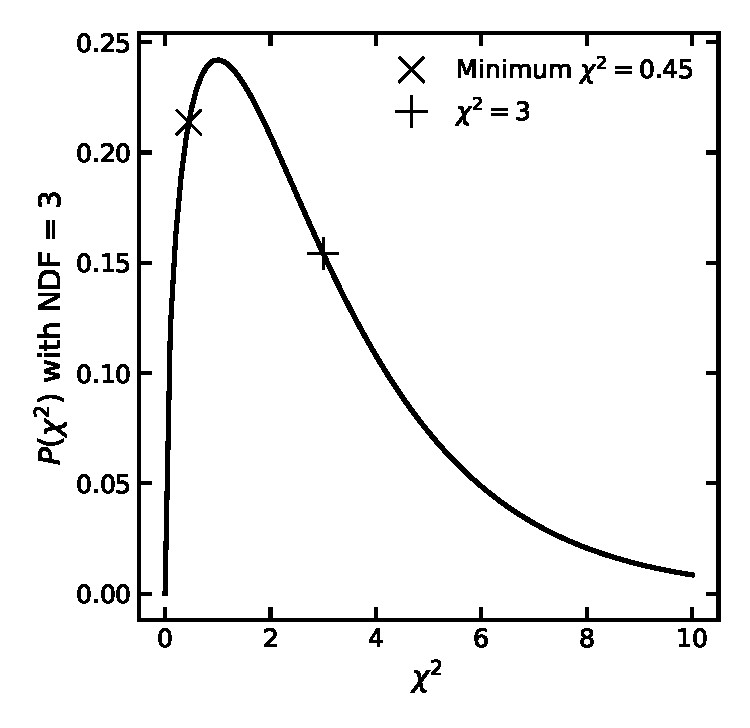
\includegraphics[width=0.5\textwidth]{ch_analysis/min_chi2_final}
    \caption[Minimum $\chi^2$ comparison]{
        Probability density function for the $\chi^2$ distribution
        with 3 degrees of freedom.
        The minimum $\chi^2$ extracted from the fitter
        is marked with an X.
        The expectation value of the minimum $\chi^2$
        for any fit with 3 degrees of freedom is 3,
        which is marked with a $+$.
    }
    \label{fig:chi2_pdf}
\end{figure}

\begin{figure}
    \centering
    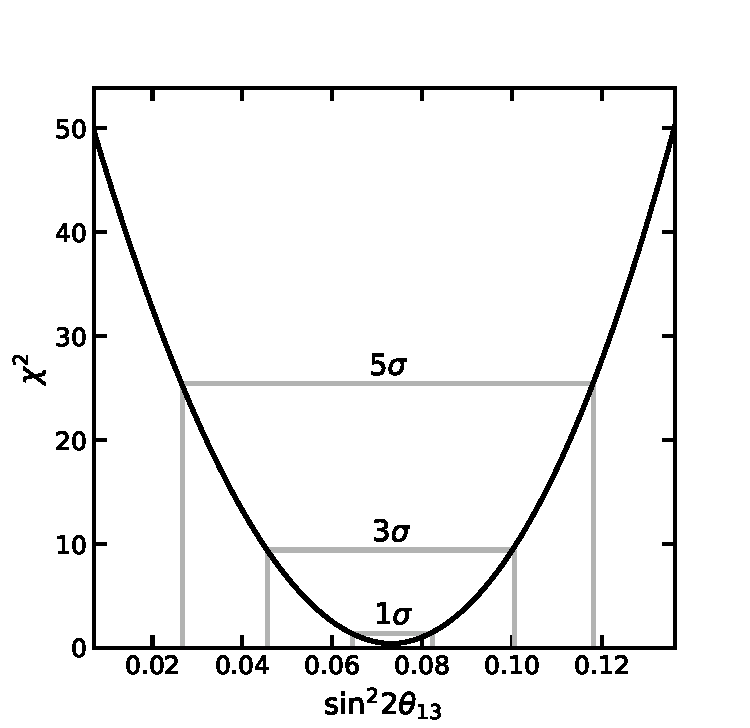
\includegraphics[width=0.5\textwidth]{ch_analysis/chi2_scan_nominal}
    \caption[$\chi^2$ scan]{
        Minimum value of $\chi^2$ as a function of $\sin^22\thetaot$.
        For each point on the curve, the value of \thetaot{} was fixed
        and the fitter minimized $\chi^2$
        using only nuisance parameters.
    }
    \label{fig:chi2_scan}
\end{figure}

The error budget for this measurement of \thetaot{}
was determined using the subtraction method \cite{nh2016technote}.
This method compares the width of the $\chi^2$ profile
with certain nuisance parameters disabled (fixed at 0)
to the width of the nominal $\chi^2$ profile
to determine the contribution of those parameters
to the final uncertainty of \thetaot{}.
This procedure was carried out directly on \thetaot{} values
rather than on $\sin^22\thetaot$.
Specifically, the effective uncertainty $\sigma$
was defined as half the range of $\thetaot$ values
producing a $\Delta \chi^2 \leq 1$.
The nominal fit with all nuisance parameters enabled
resulted in an effective uncertainty for \thetaot{} of
\begin{equation}\label{eq:nominal_unc}
    \sigma_\text{all} = \frac{0.0082 + 0.0089}{2} = 0.00855,
\end{equation}
where the two one-sided uncertainties are identical
to those quoted for \thetaot{} in \cref{eq:result}.
The uncertainty due to statistics at the far site was obtained
by disabling all pull parameters
and determining the new range for $\Delta \chi^2 \leq 1$.
This was done without the use of the minimizer since all parameters were specified,
including \thetaot{}.
For all other (systematic) sources of uncertainty $u$,
an effective uncertainty $\sigma^2_{\text{all}-u}$
was obtained by disabling only the nuisance parameters
controlling uncertainty $u$,
and performing a $\chi^2$ scan.
The final uncertainty in $\thetaot$ due to
systematic uncertainty $u$ was
\begin{equation}\label{eq:syst_error_budget}
    \sigma^2_u = \sigma^2_\text{all} - \sigma^2_{\text{all}-u}.
\end{equation}
The modified $\chi^2$ scans are shown in \cref{fig:error_budget_scans},
labeled by the pull-parameter category whose impact was tested.
Each source of uncertainty was converted into a relative contribution,
\begin{equation}\label{eq:syst_error_rel}
    f_u = \frac{\sigma^2_u}{\sigma^2_{\text{all}}}.
\end{equation}
The sum of the contributions does not equal unity
due to correlations between the effects of the uncertainties
on \thetaot{}.
The error budget is
listed in \cref{tab:error_budget}.


\begin{figure}
    \centering
    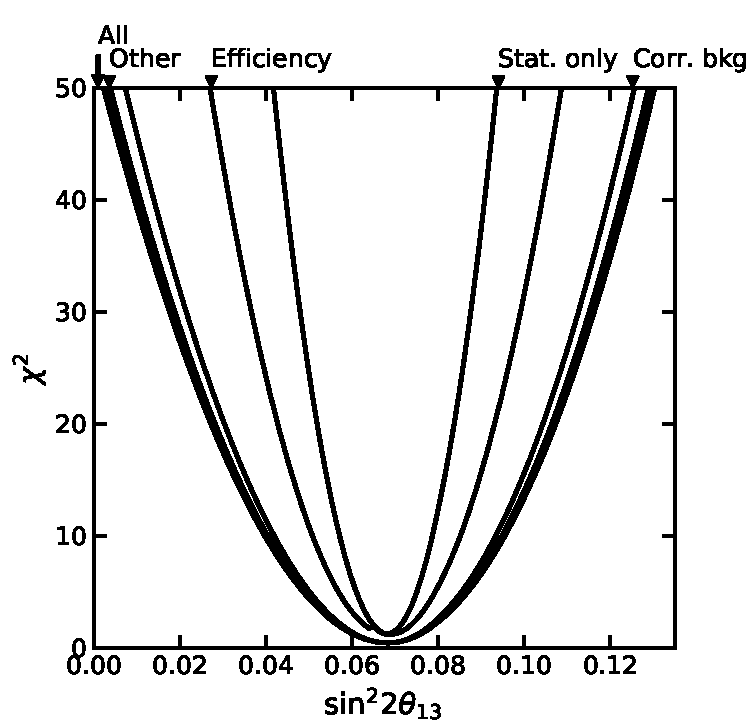
\includegraphics[width=0.5\textwidth]{ch_analysis/error_budget_chi2_scans}
    \caption[$\chi^2$ scans with disabled nuisance parameters]{
        Scans of $\chi^2$ vs. $\sin^22\thetaot$ with various nuisance parameters disabled
        in order to determine the contribution of each uncertainty
        to the total uncertainty. (See text for details.)
        The curves labeled ``All'' and ``Stat. only''
        have all pull parameters enabled and disabled, respectively.
        ``Corr. bkg.'' includes \li{}/\he{}, fast neutrons, \amc{}
        and radiogenic neutrons.
        ``Other'' is actually multiple overlapping curves,
        one for each remaining row of \cref{tab:systs}.
        Wider curves indicate a smaller contribution to the total uncertainty.
    }
    \label{fig:error_budget_scans}
\end{figure}

\begin{table}[ht]
    \centering
    \begin{tabular}[t]{lS}
        \toprule
        Uncertainty source & \parbox[t]{4cm}{
            Relative contribution\\
            $f_u = \left(%
                \sigma^2_u/\sigma^2_\text{all}%
            \right)$ [\%]
        }
        \\
        \midrule
        Statistics (EH3) & 16.01 \\
        Statistics (EH1 \& EH2) & 3.14 \\
        Detection efficiency & 54.73 \\
        Relative energy scale & 4.27 \\
        Accidental background & 1.38 \\
        \li{}/\he{} background & 14.51 \\
        Fast-neutron background & 2.21 \\
        \amc{} background & 0.94 \\
        Radiogenic neutron background & 3.57 \\
        Reactor power & 5.72 \\
        Input $\theta_{12},\Delta m^2_{21}$, and $\Delta m^2_{32}${} & 0.01 \\
        \midrule
        Total & 106.49 \\
        \bottomrule
    \end{tabular}
    \caption[Error budget]{
        Contribution of each source of uncertainty to the overall uncertainty
        of \thetaot{}.
        Listed values do not sum to \SI{100}{\percent}
        due to correlations between uncertainties.
    }
    \label{tab:error_budget}
\end{table}

To fully characterize the point in phase space
corresponding to the minimum $\chi^2$,
the best-fit values of all 184 nuisance parameters must be specified.
For convenience, the parameters are divided into
the 136 representing near site statistical uncertainties
and the 48 others, which represent the traditional systematic uncertainties.
The contribution of each pull parameter $\eta_i$ to the $\chi^2$ total
was defined (using the notation from \cref{eq:chisquare_generic}) as
\begin{equation}\label{eq:pull_contrib}
    \delta\chi^2 = \frac{\eta_i^2}{\tilde{\sigma}_{\eta,i}^2}.
\end{equation}
Since there were 136 nuisance parameters representing
the statistical fluctuations of each bin of prompt energy
in each near hall AD,
their contributions were summarized by combining the contributions
of all bins for each AD:
\begin{equation}\label{eq:pull_near_contrib}
    \delta\chi^2_{\text{near AD }i} = \sum_b \left(
        \frac{\eta_{N,i}^{(b)}}{\tilde{\sigma}_{N,i}^{(b)}}
    \right)^2.
\end{equation}
The contributions of the data-to-model comparison
(first line of \cref{eq:chisquare_full})
along with each nuisance parameter
to the total $\chi^2$
are shown in \cref{fig:syst_pulls_plot}.
16 nuisance parameters plus the 4 data-to-model comparison terms
contributed more than $10^{-6}$ to the total;
those parameters are listed with additional details
in \cref{tab:pull_details}.

\begin{figure}
    \centering
    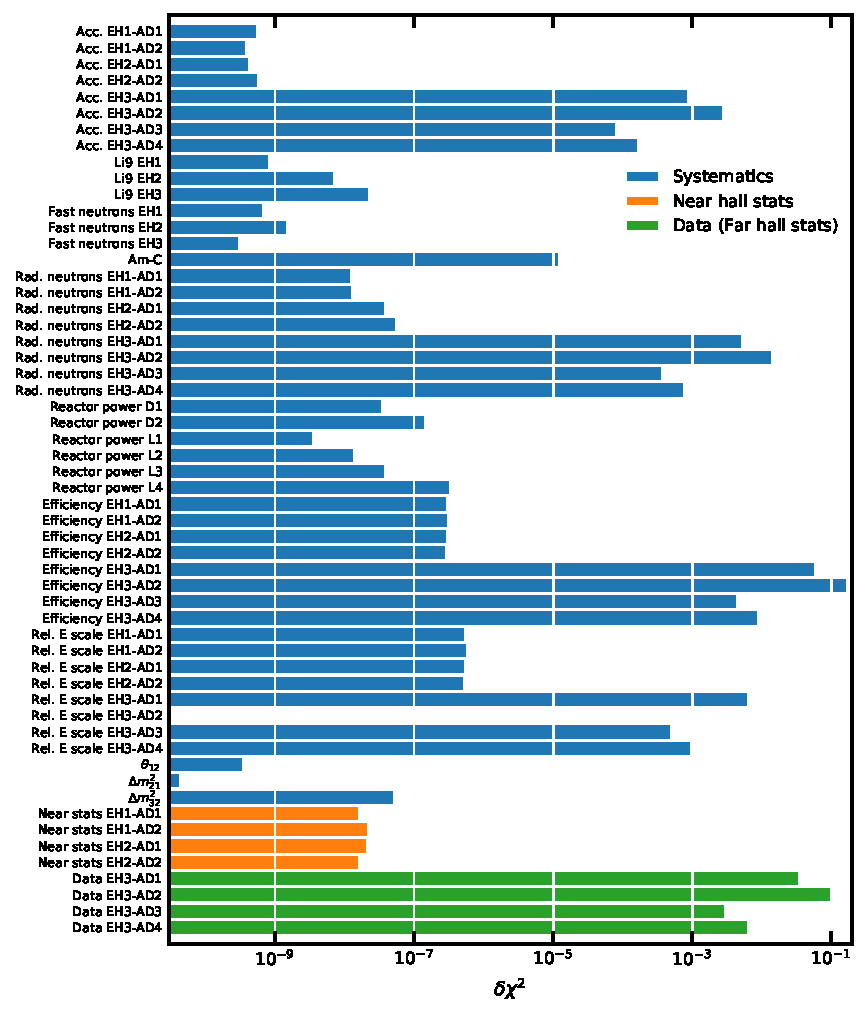
\includegraphics[height=0.9\textheight]{ch_analysis/pulls_chi2_contrib}
    \caption[Contributions to minimum $\chi^2$]{
        Contribution of each systematics nuisance parameter (blue),
        the near hall statistics nuisance parameters,
        aggregated by AD (orange),
        and the data-to-model comparison (green)
        to the total value of the minimum $\chi^2$.
    }
    \label{fig:syst_pulls_plot}
\end{figure}

\begin{table}[ht]
    \centering
    \begin{tabular}[t]{
        r
        c
        S[fixed-exponent = 0, table-omit-exponent]
        S[fixed-exponent = 0, table-omit-exponent]
        S[fixed-exponent = 0, table-omit-exponent]
    }
        \toprule
         & AD & {Best fit value} & {Constraint} & {$\delta\chi^2$} \\
        \midrule
        Data-to-model & EH3-AD1 & 161929.4 & 162005 & 0.0353 \\
        Data-to-model & EH3-AD2 & 164317.8 & 164187 & 0.104 \\
        Data-to-model & EH3-AD3 & 166349.4 & 166372 & 0.00306 \\
        Data-to-model & EH3-AD4 & 144721.5 & 144752 & 0.00642 \\
        Accidentals & EH3-AD1 & 2.41e-5 & 8.06e-4 & 8.97e-4 \\
        Accidentals & EH3-AD2 & -4.23e-5 & 7.99e-4 & 2.8e-3 \\
        Accidentals & EH3-AD3 & 7.17e-6 & 7.90e-4 & 8.23e-5 \\
        Accidentals & EH3-AD4 & 1.12e-5 & 8.57e-4 & 1.69e-4 \\
        \amc{} & Common & 0.00176 & 0.500 & 1.24e-5 \\
        Rad. neutrons & EH3-AD1 & 0.0362 & 0.5 & 0.00525 \\
        Rad. neutrons & EH3-AD2 & -0.0598 & 0.5 & 0.0143 \\
        Rad. neutrons & EH3-AD3 & 0.00961 & 0.5 & 0.000370 \\
        Rad. neutrons & EH3-AD4 & 0.0139 & 0.5 & 0.000773 \\
        Efficiency & EH3-AD1 & 0.00162 & 0.0066 & 0.0601 \\
        Efficiency & EH3-AD2 & -0.00271 & 0.0066 & 0.169 \\
        Efficiency & EH3-AD3 & 0.000445 & 0.0066 & 0.00454 \\
        Efficiency & EH3-AD4 & 0.000629 & 0.0066 & 0.00908 \\
        Rel. E scale & EH3-AD1 & 0.000403 & 0.005 & 0.00650 \\
        Rel. E scale & EH3-AD3 & 0.000112 & 0.005 & 5.01e-4 \\
        Rel. E scale & EH3-AD4 & 0.000157 & 0.005 & 9.90e-4 \\
        \bottomrule
    \end{tabular}
    \caption[Significant contributions to final $\chi^2$]{
        Details of the terms that contributed the most ($>10^{-6}$)
        to the final $\chi^2$ value of \num{0.42446}.
        For the data-to-model rows,
        the best-fit value is the model prediction for number of counts
        (including background events)
        and the constraint is the actual number of observed counts.
        The terms listed here contributed a total of \num{0.42414},
        or \SI{99.93}{\percent} of the total, to the minimum $\chi^2$.
    }
    \label{tab:pull_details}
\end{table}

%If the predictions based on different near-hall AD observations agree,
%it can be concluded that the effects due to reactor modeling
%and variation between detectors have been properly accounted for.



%For example, the number of accidental background events in a given near AD
%is estimated to be $N_{\text{acc}}$.
%In the model, this value is subtracted from the total
%observed events in that AD, $N_{\text{obs}}$.
%The expression used to account for the subtraction is,
%in simplified form,

%\begin{equation}
    %(1+\nu_{\text{obs}})N_{\text{obs}} - (1+\nu_{\text{acc}})N_{\text{acc}},
%\end{equation}
%thereby modeling both the statistical uncertainty of the near AD observation
%(as $\nu_{\text{obs}}$ is allowed to change)
%and the systematic uncertainty inherent in
%estimating the number of accidental background events
%(reflected in changes to $\nu_{\text{acc}}$).


